At this point, due to all the study and work done in the Analysis and Design phases, everything is quite well defined. Having said that, it was elaborated an implementation plan that will serve as an orientation and also as a kind of check list. Figure \ref{fig:implementation_plan} shows the implementation plan developed:

\begin{figure}[!htb]
\centerline{
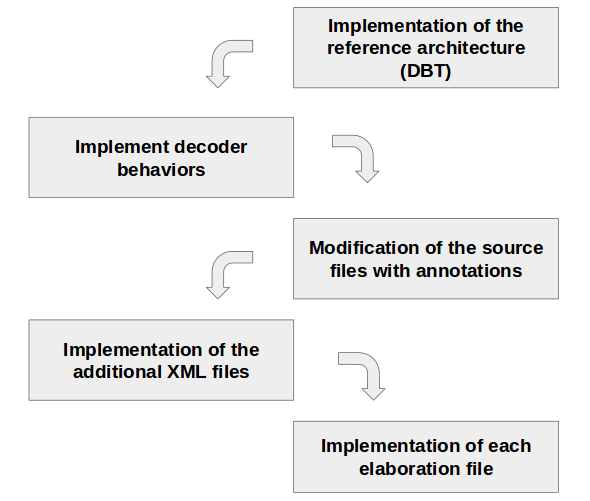
\includegraphics[scale=0.45]{images/implementation_plan}
}
\caption{Implementation Plan Diagram}
\label{fig:implementation_plan} 
\end{figure}

First of all, the groups that are committed to the DBT will implement the reference architecture using the EL language. In an initial phase, the team shall work together and discuss some common issues. Then, each group shall work independently until the global integration. 

All the decoder's behaviors explained before shall be implemented, some in hardware, some in software and some in both. The first decode based in switch cases is already implemented in the DBT. By so, only an elaboration file will be created for it. The second decode based in jump tables shall have two possible implementations: one only in software and another with some management implemented in hardware. The idea behind that is to prove the concept that two elaboration files can be created without changing the model. Also, if proved, this approach will perform accelerations in the system. However, the DBT system must be ported into an FPGA system, in this case, the Zybo Board referred in the analysis section. So, this task must also be taken. Finally, the last type of decoder (Instruction Format) will be implemented in hardware, however, will not be tested since its required a new behavior for the generator component. 

With the sources prepared, what comes next is the modification of the source files with annotations in the right locations and the creation of the elaboration files for all components of the model. Since only one of the behaviors as a configurable specific parameter (the number of bits that ensures the size of the switch cases) an additional XML file will be created in order to allow the configuration. 

